\chapter{Results}
\label{cha:results}

This chapter covers the results of the 2011 Kukui Cup competition and the experiments conducted around the competition.\fxnote{Need to list the topics covered in results}


\section{Competition Results}

The 2011 Kukui Cup competition, apart from the planned experiments, produced interesting results. This section covers those competition-level results, including changes that were made to the competition as it was underway.


\subsection{Changes During Competition}

In the course of the competition, we sometimes felt it necessary to make changes to the rules or parameters of the competition. We made these changes to to improve the competition, for example to increase participation or fairness. This section details the changes we made and the justification for each change.


\subsubsection{Energy Goal and Baseline Changes}

Before the competition, we set the energy goal for the daily Energy Goal Game (detailed in \autoref{sec:energy-goal-game}) to a 5\% reduction in energy use compared to the lounge's baseline energy use. However, for the first day of the competition, 5 of the 20 lounges met the 5\% daily energy reduction goal. Since the competition had only been running for 24 hours, with the Kickoff Party event taking place at 6:30 PM, we felt it was unlikely that the competition could have caused the change. Therefore, it seemed likely that those lounges made their goal due to random variations in energy use rather than behavioral change. For this reason, the daily energy goal was set to 10\% for the remainder of round 1 of the competition.

Due to the problems we encountered in setting initial baselines for energy use in the lounges discussed in \autoref{sec:baseline-computation}, in the interests of fairness, we decided that the baselines should be recomputed for round 2. We recomputed the baselines for each lounge based on each lounge's energy use during round 1, ensuring that the baselines were computed with a whole week of data for each lounge. For lounges that had reduced their energy use in round 1, the new baseline had the side effect of making it harder for to meet the goal, since the new baseline would be lower than the initial one. To compensate for the added difficulty, we changed the daily energy goal percentage back to 5\%. We used the new baseline and goal percentage unmodified in the final round of the competition.


\subsubsection{RA Participation}
\label{sec:ra-participation}

One question that we discussed in preparation for the competition was whether RAs should be allowed to actively participate in the competition (log into the website, earn points, and win prizes). We were concerned that if RAs could win prizes, this could demotivate the residents, who might believe that the RAs had an unfair advantage due to their position. We also felt that since the RAs were already being compensated for their work as an RA, further compensation in the form of prizes was unnecessary.

Based on this line of thought, we told RAs that they could participate in the competition, including earning points, but they would not be eligible to win prizes through either the point competition or the raffle game. RAs were to be entered into a separate RA-only drawing with unspecified but lower value prizes. 

Unfortunately, we found that after round 1, RA participation was low at 40\% (16 of 40), and in our interaction with RAs they lamented the fact that they were unable to win prizes. We decided to change course and starting on October 26 (day 3 of round 2), we made them eligible to win prizes and participate in the raffle game. RA participation after the change took effect was 62\% (23 of 37, due to some RAs attrition). In an anonymous followup survey with the RAs after the competition was over~\cite{csdl2-11-08}, prizes were listed as a common motivation for those that participated (8 of 19 responses), and confusion over the inability to win prizes was mentioned as a reason for not participating (2 of 14 responses). The survey results provide a strong indication that allowing RAs to fully participate was the correct decision and should be implemented from the beginning in future competitions.


\subsubsection{Active Participation Bonus}
\label{sec:active-participation-bonus}

In an effort to further motivate RAs to encourage their residents to participate in the competition, we instituted an additional incentive for RAs on October 26 (at the same time as the rules were changed to allow RAs to win prizes). We computed a new metric we called \emph{active participation}, which is the percentage of residents in each lounge that have earned more than 50 points in the competition. RAs were given a gift card to the UH \Manoa bookstore based on their lounge's active participation at the end of the competition: \$25 for 25\%, \$50 for 50\%, and \$100 for 100\%. To allow RAs (and others) to track their progress, a new scoreboard was added to the rotation that showed the percentage of participation for each lounge, updated in real time.

At the end of the competition, the RAs of three lounges received the \$50 bonus (for active participation of 74\%, 53\%, and 51\%), and the RAs of four lounges received the \$25 bonus (44\%, 43\%, 37\%, and 35\%).

Based on conversations with some RAs, the active participation bonus was a motivator to get their residents playing the game. However, it would likely have been more effective if it was instituted at the beginning of the competition.


\subsubsection{Referral Bonus}
\label{referral-bonus}

In an effort to increase participation in the competition, in round 2 we instituted a \emph{referral bonus}. When a participant logs into the competition website for the first time, as part of the first login process, they are asked to enter the UH email address of another participant if that other participant referred them to the competition. Once the new participant earns 30 points in the competition, then both the new participant and the existing participant are awarded 10 bonus points. New participants that successfully completed the first login process earned 25 points, so to earn the bonus, new participants had to complete at least one activity. There was no limit placed on the number of times a participant could be used as the referer.

38.3\% (159) of users logging into the competition website for the first time entered in a referring email address. Of those referred users, 93\% (148) went on to earn at least 30 points and earn the bonus. Given that the bonus was introduced in round 2, this represents a significant use of the bonus. In retrospect, it would be better for the referral bonus threshold (30 points) to be the same as the active participation bonus threshold (50 points) for consistency and to encourage additional participation.

\autoref{fig:referrals-per-referer} shows the frequency distribution of the participants making the referral. All the referrals were made by only 20 participants, and the top two referrers accounted for 66\% of all referrals made.

\begin{figure}[htbp]
	\centering
		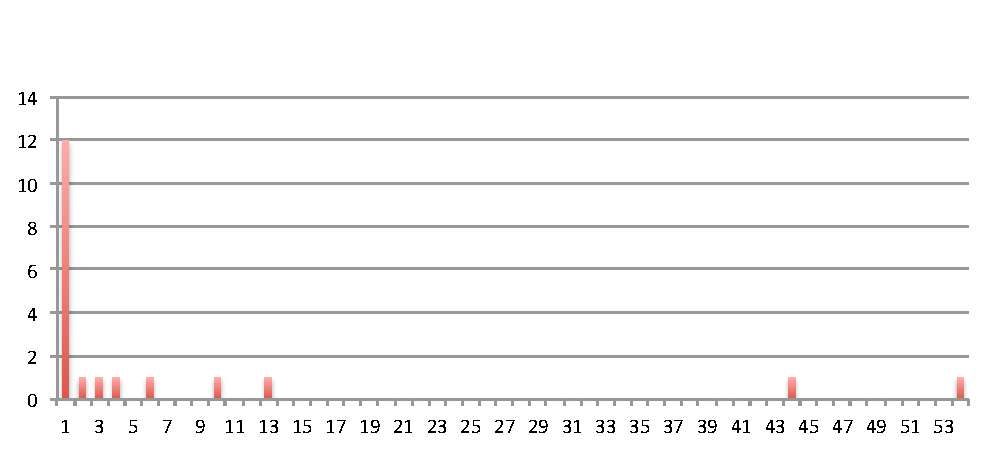
\includegraphics[scale=0.75]{referrals-per-referer-histogram}
		\caption{Number of referrals made by each participant who referred new users}\fxnote{Need axis labels}
\label{fig:referrals-per-referer}
\end{figure}

One reason for the concentration of referrals by two participants was due to the competition endgame. The overall point totals for the top two participants were very close as round 3 drew to a close. Having earned the vast majority of the points available through the Smart Grid Game, they seized on the referral bonus as an open-ended way to earn additional points. The two players attempted to sign up as many new participants as they could. On the final day, the overall winner reported that they used the participation scoreboard to determine which lounge had the lowest overall participation, and went door-to-door asking residents to log onto the competition website and complete one activity to help the referer win the competition! On the final day of the competition, there were 68 first-time users (67 matching the 25 point participation threshold discussed in \autoref{sec:participation}), and all of entered a referring email address, showing the impact of this referral bonus endgame.

\subsection{Notable Events}

%% Photo finish for round 1 energy

%% Photo finish for overall point winner

%% Stealing banners

\subsection{Winners}

%% Lounges

%% Individuals (not by name)

%% Scaffolding via staged awards
%% Competition for top in lounge prize even in final round

%% Raffle prize trading


\subsection{Raffle Game Use}


\subsection{Social Bonus Use}

It is quite likely that some participants used the social bonus for many actions to increase their scores without repeated collaboration.\fxnote{Need social bonus use data here} \fxnote{A graph of social bonus use would be good here}


\section{Participation}
\label{sec:participation}

Participation in the Kukui Cup competition was a critical measure for the evaluation of the impact of the system. All residents were indirectly participating in the energy competition since their electricity use was being monitored in aggregate, regardless of their awareness of the competition itself. However, we use the term participation here to indicate a conscious participation in the Kukui Cup, which can be measured in some way.

We use the score of each user as the metric for participation in the Kukui Cup. The competition website was the focal point of the competition it provided the only way to earn points, and the primary way to see scoreboards and information about events. When logging into the website for the first time, users are funneled through a first-login process where they must view and accept the consent form and choose a nickname. From our logs, 18 users logged into the website, but did not complete the first-login process. All users that complete the first-login process earn a minimum of 5 points, so any users that used the competition website had a non-zero score. The first-login process also displays a short introductory video and prompts the user to answer a simple question about the video to earn an additional 20 points. So most first-time users will have earned 25 points by the time they arrive at the competition website home page. Therefore, we classify any user with 25 points or more as a participant in the competition, which is conservative threshold since it only requires a single visit and no activity beyond those mandated by the first-login process.

It is possible for resident of Hale Aloha to have participated in aspects of the Kukui Cup without earning points. For example, residents could have attended events by accompanying friends or come upon them serendipitously, without submitting the paper attendance code that would allow them to earn points for attendance. Residents also could have participated by discussing sustainability topics with active participants or been lobbied to reduce energy use to improve their lounge's standings in the energy competition. Neither of these activities would have generated any evidence in the form of points in the competition. Despite these caveats, we believe a 25 point threshold is a good, minimal measure of participation.


\subsection{Individual Participation}
\label{sec:individual-participation}

According to a roster provided by Student Housing (which we used to populate user accounts for the competition website), there were 1072 residents in the Hale Aloha towers during the competition, including the 40 Resident Advisors. This number is approximate, since there were some errors in the roster, and residents sometimes move in or out of the residence halls. However, these changes are small and usually move-outs are balanced by move-ins.

Of the 1072 potential participants, 401 scored 25 points or more in the competition, for a participation rate of 37\%. However, as discussed in \autoref{referral-bonus}, on the final day of the competition there were 67 new participants who were persuaded to participate by a concerted effort by a small number of users to increase their score through referral bonuses. While these final-day participants may have learned more about energy through their participation in online activities, by participating for less than a day they probably did not contribute significantly to energy conservation efforts in their lounge. The participation rate without this final day surge, the participation rate would be 31\%. \autoref{fig:participants-over-time} shows how the number of new and total participants varied over the competition period.

\begin{figure}[htbp]
	\centering
		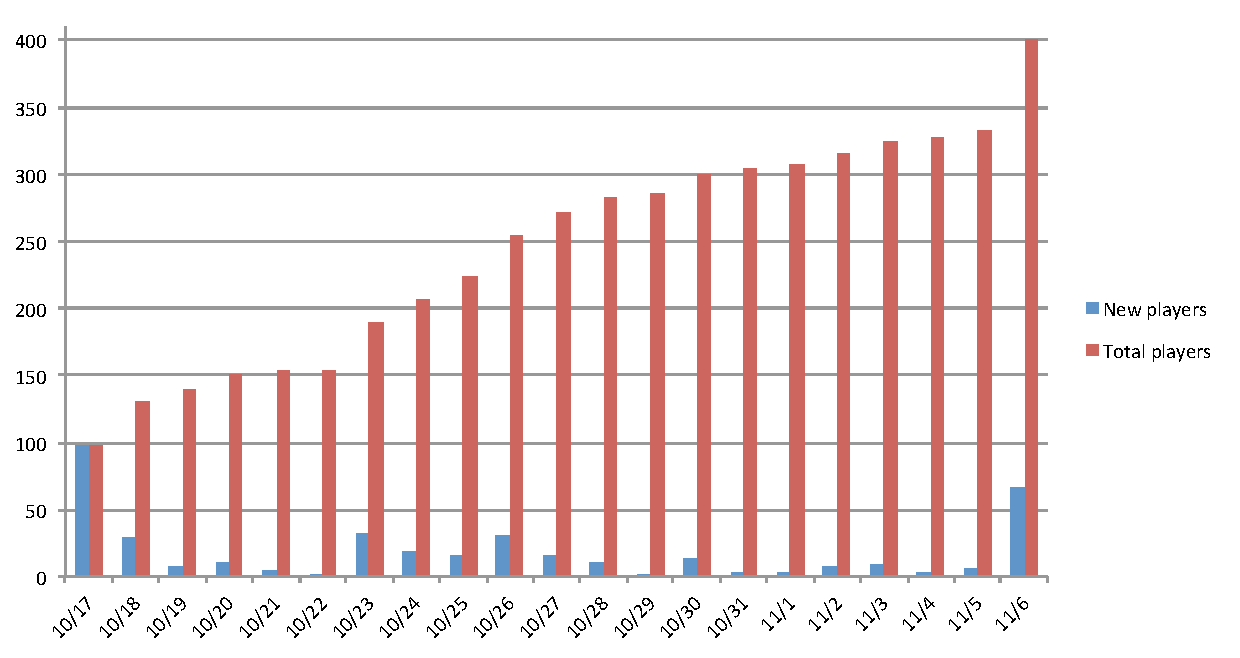
\includegraphics[scale=0.8]{participants-over-time}
		\caption{Number of new and total participants per day of competition}
\label{fig:participants-over-time}
\end{figure}


\subsection{Lounge Participation}

Using the same 25 point participation threshold, we can compute the aggregate participation rate for each lounge. \autoref{tab:lounge-participation} shows the participation rate and total score for each lounge at the end of each of the three rounds of the competition. The lounges that won the point competition for each round are shown in bold. This table shows the significant disparities in participation between lounges, with three lounges participating at 15\% or less, and the with the best lounge participating at 74\%.

%% Using \multicolumn to make spanning columns & to remove border from 1st cell
\begin{table}[htbp]
	\centering
		\begin{tabular}{ l | c | r | c | r | c | r |}
			\cline{2-7}
			 & \multicolumn{2}{c|}{Round 1} & \multicolumn{2}{c|}{Round 2} & \multicolumn{2}{c|}{Overall round} \\ \hline
			\multicolumn{1}{|l|}{Lounge} & Participation & Score & Participation & Score & Participation & Score \\ \hline \hline
			\multicolumn{1}{|l|}{Ilima-A} & 37\% & 5152 & 69\% & \textbf{9045} & 74\% & \textbf{12840} \\ \hline
			\multicolumn{1}{|l|}{Ilima-B} & 19\% & 755 & 26\% & 1480 & 35\% & 2248 \\ \hline
			\multicolumn{1}{|l|}{Ilima-C} & 11\% & 754 & 13\% & 1149 & 15\% & 1472 \\ \hline
			\multicolumn{1}{|l|}{Ilima-D} & 13\% & 264 & 22\% & 1026 & 26\% & 1469 \\ \hline
			\multicolumn{1}{|l|}{Ilima-E} & 11\% & 406 & 11\% & 681 & 13\% & 1251 \\ \hline
			\multicolumn{1}{|l|}{Lehua-A} & 7\% & 373 & 15\% & 899 & 15\% & 1493 \\ \hline
			\multicolumn{1}{|l|}{Lehua-B} & 19\% & 1831 & 24\% & 3208 & 44\% & 5214 \\ \hline
			\multicolumn{1}{|l|}{Lehua-C} & 13\% & 1140 & 24\% & 2736 & 31\% & 3868 \\ \hline
			\multicolumn{1}{|l|}{Lehua-D} & 33\% & 4898 & 37\% & 6855 & 44\% & 8963 \\ \hline
			\multicolumn{1}{|l|}{Lehua-E} & 43\% & \textbf{5288} & 44\% & 6837 & 52\% & 7702 \\ \hline
			\multicolumn{1}{|l|}{Lokelani-A} & 17\% & 389 & 56\% & 3019 & 67\% & 5087 \\ \hline
			\multicolumn{1}{|l|}{Lokelani-B} & 13\% & 455 & 20\% & 623 & 30\% & 1219 \\ \hline
			\multicolumn{1}{|l|}{Lokelani-C} & 24\% & 1344 & 31\% & 1942 & 35\% & 2391 \\ \hline
			\multicolumn{1}{|l|}{Lokelani-D} & 11\% & 335 & 15\% & 972 & 26\% & 1585 \\ \hline
			\multicolumn{1}{|l|}{Lokelani-E} & 15\% & 1989 & 19\% & 2838 & 22\% & 3858 \\ \hline
			\multicolumn{1}{|l|}{Mokihana-A} & 15\% & 745 & 37\% & 2565 & 54\% & 4436 \\ \hline
			\multicolumn{1}{|l|}{Mokihana-B} & 13\% & 994 & 19\% & 1831 & 31\% & 3427 \\ \hline
			\multicolumn{1}{|l|}{Mokihana-C} & 6\% & 328 & 17\% & 826 & 37\% & 1501 \\ \hline
			\multicolumn{1}{|l|}{Mokihana-D} & 7\% & 574 & 19\% & 1844 & 37\% & 4351 \\ \hline
			\multicolumn{1}{|l|}{Mokihana-E} & 24\% & 2104 & 39\% & 5422 & 54\% & 8837 \\ \hline
		\end{tabular}
	\caption[Score and participation per lounge at the end of each round]{Score and participation per lounge at the end of each round, bold entries indicate round winners}
\label{tab:lounge-participation}
\end{table}

As discussed in \autoref{sec:individual-participation}, the final day surge of participants inflates the participation rate of lounges. \autoref{tab:lounge-minus-endgame} shows the final participation rates with and without the final day surge, while \autoref{fig:lounge-participation} shows a plot ordered by participation rate. The participation rate without the final surge is more appropriate when the participation is being compared to other data, such as energy use, which would not have been significantly impacted by participants who joined on the final day of the competition.

\begin{table}[htbp]
	\centering
		\begin{tabular}{| l | c | c |}
			\hline
			Lounge & Overall participation & Minus final day \\ \hline
			Ilima-A & 74\% & 69\% \\ \hline
			Ilima-B & 35\% & 26\% \\ \hline
			Ilima-C & 15\% & 13\% \\ \hline
			Ilima-D & 26\% & 22\% \\ \hline
			Ilima-E & 13\% & 11\% \\ \hline
			Lehua-A & 15\% & 15\% \\ \hline
			Lehua-B & 44\% & 31\% \\ \hline
			Lehua-C & 31\% & 26\% \\ \hline
			Lehua-D & 44\% & 39\% \\ \hline
			Lehua-E & 52\% & 50\% \\ \hline
			Lokelani-A & 67\% & 63\% \\ \hline
			Lokelani-B & 30\% & 22\% \\ \hline
			Lokelani-C & 35\% & 33\% \\ \hline
			Lokelani-D & 26\% & 19\% \\ \hline
			Lokelani-E & 22\% & 19\% \\ \hline
			Mokihana-A & 54\% & 54\% \\ \hline
			Mokihana-B & 31\% & 24\% \\ \hline
			Mokihana-C & 37\% & 24\% \\ \hline
			Mokihana-D & 37\% & 20\% \\ \hline
			Mokihana-E & 54\% & 39\% \\ \hline
		\end{tabular}
	\caption{Overall Lounge participation with and without final day surge}
\label{tab:lounge-minus-endgame}
\end{table}

\begin{figure}[htbp]
	\centering
		\includegraphics[width=\textwidth]{lounge-participation}
		\caption{Plot of overall Lounge participation with and without final day surge}
\label{fig:lounge-participation}
\end{figure}


\section{Energy Literacy}

As discussed in \autoref{sec:exp-literacy-questionnaire}, I administered an online energy literacy questionnaire to a set of residents in Hale Aloha twice: once before the competition, and once after the competition. This section covers the results from those questionnaires. The full text of the questions can be found in \autoref{app:energy-literacy}.

\subsection{Questionnaire Responses}

Since each subject was to be compensated for participating in the questionnaire, and I did not know beforehand how many potential subjects would actually participate, I sent the questionnaire invitation in two waves. The first wave of 74 email invitations was sent on October 5, 2011, and a second wave of 107 invitations was sent on October 10. 68 questionnaires were completed, which is a response rate of 38\%. There were 5 partial responses, but in each case the subjects abandoned the survey before submitting any data other than the informed consent page, I have not included those subjects in the following analyses.

After the competition was complete, I sent the same questionnaire to all the individuals that had participated in the pre-competition questionnaire. There were 51 complete responses, and 2 responses that stopped after filling out the consent form. Since the questionnaire was administered before the competition began, I could not tell in advance how many subjects would go on to participate in the competition. As discussed in \autoref{sec:participation}, I call subjects participants if they earned 25 points in the competition. \autoref{tab:questionnaire-responses} shows the number of questionnaire responses from participants and non-participants, and those that completed both questionnaires. 48 subjects completed both the pre-competition and post-competition questionnaires, evenly split between participants and non-participants.

\begin{table}[htbp]
	\centering
		\begin{tabular}{| l | c | c | c |}
			\hline
			Subject type & Pre-competition & Post-competition & Completed both \tabularnewline \hline \hline
			Non-competition participants & 36 & 27 & 24 \tabularnewline \hline
			Competition participants & 32 & 24 & 24 \tabularnewline \hline \hline
			Total & 68 & 51 & 48 \tabularnewline \hline
		\end{tabular}
	\caption{Number of completed pre- and post-competition questionnaires}
\label{tab:questionnaire-responses}
\end{table}


\subsection{Energy Knowledge}

The energy knowledge section of the questionnaire consisted of 19 factual questions about energy, with a specific emphasis on \Hawaii energy issues. \autoref{tab:knowledge-descriptives} shows the average number of questions answered correctly for participants and non-participants in the pre and post-competition questionnaires. Non-participants showed a tiny reduction in questions answered correctly after the competition, while participants improved by 18.8\%. \autoref{fig:knowledge-anova} is a plot of the results.

\begin{table}[htbp]
	\centering
		\begin{tabular}{ l | c | c | c | c | c }
			\cline{2-5}
			& \multicolumn{2}{c |}{Pre-competition} & \multicolumn{2}{c|}{Post-competition} & \\ \hline
			\multicolumn{1}{|l|}{Subject type} & Mean & Std. Deviation & Mean & Std. Deviation & \multicolumn{1}{c|}{\% Change} \tabularnewline \hline \hline
			\multicolumn{1}{|l|}{Non-competition participants} & 7.46 & 2.377 & 7.37 & 2.570 & \multicolumn{1}{c|}{-1.2\%} \tabularnewline \hline
			\multicolumn{1}{|l|}{Competition participants} & 7.54 & 1.837 & 8.96 & 3.290 & \multicolumn{1}{c|}{18.8\%} \tabularnewline \hline
		\end{tabular}
	\caption[Energy knowledge before and after competition]{Average number of energy knowledge questions correct for participants and non-participants before and after the competition}
\label{tab:knowledge-descriptives}
\end{table}

\begin{figure}[htbp]
	\centering
		\includegraphics[width=0.6\textwidth]{knowledge-anova.eps}
		\caption[Plot of energy knowledge before and after competition]{Plot of average number of energy knowledge questions correct for participants and non-participants before and after the competition}
\label{fig:knowledge-anova}
\end{figure}

Using ANOVA, there was a significant interaction between participation and differences between pre and post-competition scores, \(F(1, 46) = 3.84\), \(p = 0.056\), MSE \(= 3.52\). This supports the hypothesis that participating in the Kukui Cup increases the energy literacy of participants.

\begin{figure}[htbp]
	\centering
		\includegraphics[width=\textwidth]{knowledge-questions.eps}
		\caption[Plot of energy knowledge before and after competition]{Percentage of correct answers for each energy knowledge question}
\label{fig:knowledge-questions}
\end{figure}

\autoref{fig:knowledge-questions} shows the percentage of subjects that correctly answered each of the 19 questions in the energy literacy section, from most correct to least correct. The full text of each question can be found in \autoref{sec:knowledge-items}. The following sections break down the questions by knowledge area.


\subsubsection{Climate Change}

\autoref{fig:knowledge-climate-change} shows the percentage of climate change questions answered correctly by subjects. Subjects appear to have a good understanding of climate change in general (more than 90\% knew the effects of climate change, and more than 75\% knew the cause), though most don't know precise \COtwo levels (15--20\% correct). This suggests that the climate change portions of the Kukui Cup educational content can focus less on basic information, and spend more time on specifics such as \COtwo levels in the atmosphere.

\begin{figure}[htbp]
	\centering
		\includegraphics[width=\textwidth]{knowledge-climate-change.eps}
		\caption{Percentage of correct answers for climate change questions}
\label{fig:knowledge-climate-change}
\end{figure}


\subsubsection{\Hawaii Topics}

\autoref{fig:knowledge-hawaii} shows the percentage of questions directly about \Hawaii answered correctly by subjects. For the critical question of where most of \Hawaii's energy comes from, only half of subjects knew that it comes primarily from oil. Even fewer knew how much energy an average home in \Hawaii uses (20 \kWh), an important part of developing intuition about energy use. Knowledge of the goals of the \Hawaii Clean Energy Initiative (HCEI) was the lowest of any question in the literature section. Since the HCEI is a major part of \Hawaii's renewable energy policy, competitions should find ways to make participants more aware of the HCEI goals.

\begin{figure}[htbp]
	\centering
		\includegraphics[width=\textwidth]{knowledge-hawaii.eps}
		\caption{Percentage of correct answers for climate change questions}
\label{fig:knowledge-hawaii}
\end{figure}

%% Need to continue with rest of questions




%\begin{table}[htbp]
%	\centering
%		\begin{tabular}{ l l | c | c || c | c || c | c |}
%			\cline{3-8}
%			& & \multicolumn{2}{c ||}{Non-participant} & \multicolumn{2}{c||}{Participant} & \multicolumn{2}{c|}{Total} \\ \hline
%			\multicolumn{1}{|l|}{Question \#} & Question summary & Pre & Post & Pre & Post & Pre & \multicolumn{1}{c|}{Post} \tabularnewline \hline \hline
%			\multicolumn{1}{|l|}{Q1} & Power unit & 31\% & 22\% & 34\% & 46\% & 32\% & 33\% \tabularnewline \hline
%			\multicolumn{1}{|l|}{Q3} & Energy unit & 14\% & 22\% & 13\% & 29\% & 13\% & 25\% \tabularnewline \hline
%			\multicolumn{1}{|l|}{Q12} & CFL energy calc. & 64\% & 63\% & 69\% & 63\% & 66\% & 63\% \tabularnewline \hline
%			\multicolumn{1}{|l|}{Q13} & Game console energy calc. & 19\% & 11\% & 19\% & 29\% & 19\% & 20\% \tabularnewline \hline
%			\multicolumn{1}{|l|}{Q5a} & incandescent bulb & 50\% & 63\% & 53\% & 63\% & 51\% & 63\% \tabularnewline \hline
%			\multicolumn{1}{|l|}{Q5b} & CFL & 50\% & 48\% & 31\% & 50\% & 41\% & 49\% \tabularnewline \hline
%			\multicolumn{1}{|l|}{Q5c} & LED & 44\% & 48\% & 38\% & 58\% & 41\% & 53\% \tabularnewline \hline
%			\multicolumn{1}{|l|}{Q7a} & desk lamp & 33\% & 19\% & 13\% & 25\% & 24\% & 22\% \tabularnewline \hline
%			\multicolumn{1}{|l|}{Q7b} & mobile phone charger & 36\% & 30\% & 22\% & 25\% & 29\% & 27\% \tabularnewline \hline
%			\multicolumn{1}{|l|}{Q7c} & plasma TV & 22\% & 48\% & 28\% & 46\% & 25\% & 47\% \tabularnewline \hline
%			\multicolumn{1}{|l|}{Q7d} & microwave & 28\% & 30\% & 38\% & 67\% & 32\% & 47\% \tabularnewline \hline
%			\multicolumn{1}{|l|}{Q7e} & laptop & 44\% & 48\% & 47\% & 54\% & 46\% & 51\% \tabularnewline \hline
%			\multicolumn{1}{|l|}{Q8} & Daily home energy use & 17\% & 22\% & 13\% & 21\% & 15\% & 22\% \tabularnewline \hline
%			\multicolumn{1}{|l|}{Q9} & solar panel power & 42\% & 22\% & 38\% & 29\% & 40\% & 25\% \tabularnewline \hline
%			\multicolumn{1}{|l|}{Q11} & Hawaii's electricity source & 42\% & 33\% & 56\% & 79\% & 49\% & 55\% \tabularnewline \hline
%			\multicolumn{1}{|l|}{Q4} & HCEI goal & 6\% & 7\% & 3\% & 17\% & 4\% & 12\% \tabularnewline \hline
%			\multicolumn{1}{|l|}{Q2} & Climate change cause & 69\% & 67\% & 91\% & 83\% & 79\% & 75\% \tabularnewline \hline
%			\multicolumn{1}{|l|}{Q10} & Climate change effects & 92\% & 96\% & 91\% & 92\% & 91\% & 94\% \tabularnewline \hline
%			\multicolumn{1}{|l|}{Q6} & CO2 levels & 8\% & 19\% & 22\% & 21\% & 15\% & 20\% \tabularnewline \hline
%		\end{tabular}
%	\caption[Energy knowledge before and after competition]{Average number of energy knowledge questions correct for participants and non-participants before and after the competition}
%\label{tab:knowledge-correct}
%\end{table}



\subsection{Energy Attitudes}

The energy attitudes section of the questionnaire was taken from the affective subscale of the energy literacy questionnaire developed by DeWaters and Powers~\cite{DeWaters2011}. There are 18 statements in the attitudes section using a five-point Likert scale from 1 for ``strongly agree'' to 5 for ``strongly disagree''. \autoref{tab:attitude-descriptives} shows the average rating value across all 18 statements for participants and non-participants in the pre and post-competition questionnaires. \autoref{fig:attitude-anova} is a plot of the results.

\begin{table}[htbp]
	\centering
		\begin{tabular}{ l | c | c | c | c | c }
			\cline{2-5}
			& \multicolumn{2}{c |}{Pre-competition} & \multicolumn{2}{c|}{Post-competition} & \\ \hline
			\multicolumn{1}{|l|}{Subject type} & Mean & Std. Deviation & Mean & Std. Deviation & \multicolumn{1}{c|}{\% Improvement} \tabularnewline \hline \hline
			\multicolumn{1}{|l|}{Non-competition participants} & 2.23 & 0.438 & 2.11 & 0.561 & \multicolumn{1}{c|}{5.5\%} \tabularnewline \hline
			\multicolumn{1}{|l|}{Competition participants} & 2.11 & 0.428 & 2.13 & 0.719 & \multicolumn{1}{c|}{-0.8\%} \tabularnewline \hline
		\end{tabular}
	\caption[Energy attitudes before and after competition]{Average energy attitude scores for participants and non-participants before and after the competition}
\label{tab:attitude-descriptives}
\end{table}

\begin{figure}[htbp]
	\centering
		\includegraphics[width=0.7\textwidth]{attitude-percent-anova}
		\caption[Plot of energy attitudes before and after competition]{Plot of average energy attitude scores for participants and non-participants before and after the competition}
\label{fig:attitude-anova}
\end{figure}

Non-participants showed a small improvement in their attitude score in the post-competition questionnaire, while participants scores decreased slightly, but these results were not statistically significant. These results indicate that the 2011 Kukui Cup did not change the attitude of participants towards energy conservation and renewable energy. It may be that the three week competition length was not long enough to change attitudes, or perhaps the competition's focus on direct energy conservation actions took away from potential changes in attitude.

\fxnote{Add comparison to DeWaters results}

%\begin{table}[htbp]
%	\centering
%	\scriptsize
%		\begin{tabular}{| p{5cm} | >{\centering}p{1.4cm} | c | c | c | >{\centering}p{1.1cm} | >{\centering}p{1.3cm} | c |}
%			\hline
%			Question & Strongly \newline disagree (5) & Disagree (4) & Neutral (3) & Agree (2) & Strongly \newline agree (1) & Choose not \newline to answer & Average \tabularnewline \hline \hline
%			Energy education should be an important part of every school's curriculum. & 0 (0\%) & 5 (7.4\%) & 27 (39.7\%) & 20 (29.4\%) & 14 (20.6\%) & 2 (2.9\%) & 2.35 \tabularnewline \hline
%			I would do more to save energy if I knew how. & 3 & 4 & 9 & 33 & 18 & 1 & 2.12 \tabularnewline \hline
%			Saving energy is important. & 1 & 1 & 4 & 24 & 37 & 1 & 1.58 \tabularnewline \hline
%		\end{tabular}
%	\caption{Pre-competition energy attitude responses}
%\label{tab:pre-energy-attitude}
%\end{table}


\subsection{Reported Energy Behaviors}

The energy behavior section of the questionnaire consisted of 17 statements about energy use behaviors inspired by the energy literacy instrument developed by DeWaters and Powers~\cite{DeWaters2011}. Each statement was rated on a scale from 1 for ``always or almost always'' to 5 for ``never or hardly ever''. \autoref{tab:behavior-descriptives} shows the average rating value across all 17 statements for participants and non-participants in the pre and post-competition questionnaires. Non-participants showed a small improvement in their behavior score in the post-competition questionnaire, with participants showing a slightly larger improvement. \autoref{fig:behavior-anova} is a plot of the results.

\begin{table}[htbp]
	\centering
		\begin{tabular}{ l | c | c | c | c | c }
			\cline{2-5}
			& \multicolumn{2}{c |}{Pre-competition} & \multicolumn{2}{c|}{Post-competition} & \\ \hline
			\multicolumn{1}{|l|}{Subject type} & Mean & Std. Deviation & Mean & Std. Deviation & \multicolumn{1}{c|}{\% Improvement} \tabularnewline \hline \hline
			\multicolumn{1}{|l|}{Non-competition participants} & 2.56 & 0.510 & 2.52 & 0.596 & \multicolumn{1}{c|}{1.7\%} \tabularnewline \hline
			\multicolumn{1}{|l|}{Competition participants} & 2.52 & 0.443 & 2.35 & 0.339 & \multicolumn{1}{c|}{6.6\%} \tabularnewline \hline
		\end{tabular}
	\caption[Reported energy behaviors before and after competition]{Average self-reported energy behavior scores for participants and non-participants before and after the competition}
\label{tab:behavior-descriptives}
\end{table}

\begin{figure}[htbp]
	\centering
		\includegraphics[width=0.7\textwidth]{behavior-anova.eps}
		\caption[Plot of energy behavior before and after competition]{Plot of average self-reported energy behavior scores for participants and non-participants before and after the competition}
\label{fig:behavior-anova}
\end{figure}

Using ANOVA, there was a significant difference\fxnote{Correct terminology here?} between pre and post-competition scores, \(F(1, 46) = 4.09\), \(p = 0.049\), MSE \(= 2.94\), but interaction between participation and pre and post-competition scores was not significant. Since the self-reports of behavior changes took place for both participants and non-participants, this provides the interesting possibility of \emph{passive participants} who made changes in their behavior due to the competition, but did not participate in the competition (based on my definition participation: earning 25 points). Since most of the targeted behaviors are public and some involve shared resources (such as the overhead lighting in residents' rooms), it is not hard to imagine that non-participants might find themselves changing their behaviors due to requests from roommates who are participating, or new social norms developing as a result of participants behavior. Future iterations of the Kukui Cup could encourage these changes in behavior even among non-participants through additional activities that target non-participants (``get your roommate to take the stairs'') or additional marketing materials designed around establishing new social norms as described in \autoref{sec:norms}.


\subsection{Group Identification}

I used the Arrow-Carini Group Identification Scale 2.0~\cite{Henry1999} for the group identification section of the questionnaire. It consists of 12 statements in three subscales: affective, behavioral, and cognitive. Subjects were asked to respond to each one on a seven-point Likert scale from 1 for strongly disagree to 7 for strongly agree. The group specified in the statements was the lounge that subjects belong to, since lounges represent the teams in the Kukui Cup. \autoref{tab:group-id-descriptives} shows the average scale value for participants and non-participants in the pre and post-competition questionnaires, while \autoref{fig:group-id-anova} shows a plot of the results.

\begin{table}[htbp]
	\centering
		\begin{tabular}{ l | c | c | c | c | c }
			\cline{2-5}
			& \multicolumn{2}{c |}{Pre-competition} & \multicolumn{2}{c|}{Post-competition} & \\ \hline
			\multicolumn{1}{|l|}{Subject type} & Mean & Std. Deviation & Mean & Std. Deviation & \multicolumn{1}{c|}{\% Change} \tabularnewline \hline \hline
			\multicolumn{1}{|l|}{Non-competition participants} & 4.10 & 0.869 & 4.14 & 0.872 & \multicolumn{1}{c|}{1.0\%} \tabularnewline \hline
			\multicolumn{1}{|l|}{Competition participants} & 4.13 & 0.823 & 3.79 & 0.963 & \multicolumn{1}{c|}{-8.0\%} \tabularnewline \hline
		\end{tabular}
	\caption[Group identity score before and after competition]{Average group identification scores for participants and non-participants before and after the competition}
\label{tab:group-id-descriptives}
\end{table}

\begin{figure}[htbp]
	\centering
		\includegraphics[width=0.7\textwidth]{group-id-anova.eps}
		\caption[Plot of group identification before and after competition]{Plot of average group identification scores for participants and non-participants before and after the competition}
\label{fig:group-id-anova}
\end{figure}

Both participants and non-participants were neutral towards their lounge. Participants showed a decline of 8\% in their group identification with the lounge, while non-participants were mostly unchanged. These results were not statistically significant, but they provide interesting possibilities to be investigated further. While I had hypothesized that the Kukui Cup experience would increase participants' identification with the lounge, it may be that participants started to identify with other Kukui Cup participants rather than fellow loungemates. Another possible scenario could be that dedicated participants who are trying to reduce their lounge's energy use might find themselves alienated from their loungemates who are not making an effort to conserve energy.

It is worth noting that two subjects indicated in the questionnaire feedback that they did not know what a lounge was (see \autoref{questionnaire-feedback}), and all the group identification statements referred to the subjects' lounge. It is possible that other subjects also did not understand the lounge grouping, which could explain the neutral ranking and lack of significant change after the competition.


\subsection{Connectedness to Nature}

I used the connectedness to nature section of the questionnaire, I used the scale developed by Mayer and Frantz~\cite{MayerFrantz2004}. It consists of 14 statements regarding the relationship between humans and nature. Subjects were asked to respond to each statement on a five-point Likert scale from 1 for strongly disagree to 5 for strongly agree. \autoref{tab:cns-descriptives} shows the average scale value for participants and non-participants in the pre and post-competition questionnaires, while \autoref{fig:cns-anova} shows a plot of the results.

\begin{table}[htbp]
	\centering
		\begin{tabular}{ l | c | c | c | c | c }
			\cline{2-5}
			& \multicolumn{2}{c |}{Pre-competition} & \multicolumn{2}{c|}{Post-competition} & \\ \hline
			\multicolumn{1}{|l|}{Subject type} & Mean & Std. Deviation & Mean & Std. Deviation & \multicolumn{1}{c|}{\% Change} \tabularnewline \hline \hline
			\multicolumn{1}{|l|}{Non-competition participants} & 3.39 & 0.822 & 3.55 & 0.794 & \multicolumn{1}{c|}{4.4\%} \tabularnewline \hline
			\multicolumn{1}{|l|}{Competition participants} & 3.47 & 0.547 & 3.51 & 0.602 & \multicolumn{1}{c|}{1.1\%} \tabularnewline \hline
		\end{tabular}
	\caption[CNS score before and after competition]{Average connectedness to nature scores for participants and non-participants before and after the competition}
\label{tab:cns-descriptives}
\end{table}

\begin{figure}[htbp]
	\centering
		\includegraphics[width=0.7\textwidth]{cns-anova.eps}
		\caption[Plot of CNS results before and after competition]{Plot of average connectedness-to-nature scores for participants and non-participants before and after the competition}
\label{fig:cns-anova}
\end{figure}

Using ANOVA, there was a significant difference\fxnote{Correct terminology here?} between pre and post-competition scores, \(F(1, 46) = 3.85\), \(p = 0.056\), MSE \(= 2.61\), but interaction between participation and pre and post-competition scores was not significant. However, the CNS scale was intended to be used to determine whether lounges with higher aggregate CNS scores were

%% STOPPED HERE

\subsection{Questionnaire Feedback}
\label{questionnaire-feedback}

At the end of both questionnaires, subjects were given the opportunity to provide feedback about the questionnaire in an optional free response question. There were 12 feedback responses to the pre-competition questionnaire, and 5 to the post-competition questionnaire (excluding non-responses such as ``N/A'' and ``No comment :)''). \autoref{tab:questionnaire-feedback} shows a summary of the responses. Note that some subjects' feedback spanned multiple categories, so the number of responses in the table is greater than the number of subjects.

\begin{table}[htbp]
	\centering
		\begin{tabular}{| l | c | c | p{4.5cm}|}
			\hline
			Type of response & Pre-competition & Post-competition & Example response \\ \hline \hline
			Accolade & 1 & 2 & ``Great Survey!'' \\ \hline
			General confusion & 3 & & ``I am confused... But I did it!'' \\ \hline
			Lounge confusion & 2 & 1 (same subject) & ``The questions about the `lounge' were very confusing. I assumed it was about the other members of where I am living but I'm not completely sure.'' \\ \hline
			Long questionnaire & 1 & & ``its long'' \\ \hline
			Importance of energy & & 2 & ``Saving energy is very important'' \\ \hline
			Questionnaire concerns & 2 & 1 & ``\ldots I do not understand why half of the questions from the lounge section were reworded versions of the first half.'' \\ \hline
			Energy introspection & 2 & & ``this survey made me think. i feel more aware now that i could do more to save energy.'' \\ \hline
			Other & 2 & & ``I am one with nature. I am one with the lounge.'' \\ \hline
		\end{tabular}
	\caption{Summary of free-response questionnaire feedback}
\label{tab:questionnaire-feedback}
\end{table}

While only a small number of subjects provided feedback, the results show a range of responses to the questionnaire. Two subjects indicated that they were unsure what a lounge was, demonstrating that understanding of the lounge as an entity was not universal among subjects (one subject indicated this on both pre and post-competition questionnaires, so two subjects account for the three responses listed in the table). Two subjects indicated that the questionnaire made them more aware of ways they could conserve energy. If they actually followed through with behavior changes, the effectiveness of future Kukui Cup iterations could be improved by administering the pre-competition questionnaire to a greater percentage of residents. This would also mean that the questionnaire itself could have resulted in attitude or behavior changes.

\section{Energy Use}

%% baseline recommendation for Campus Conservation Nationals: 2 weeks before 3 week-long competition.

\subsection{Before Competition}


\subsection{During Competition}

\subsection{Energy Goal Game}

Participants from the highest-scoring lounges realized that meeting the daily goal greatly increased their lounge's score (since each active participant received 20 points), motivating them to continue to 

\subsection{After Competition}








\section{Post-Competition Energy Audit}
\label{sec:post-energy-audit}

As described in \autoref{sec:meter-installation}, installation of the electricity meters for the competition was completed during the Fall 2011 semester. A joint team from UH \Manoa Student Housing and the Kukui Cup project conducted an energy audit of the four Hale Aloha towers during the winter break after the Fall 2011 semester~\cite{csdl2-11-12}. Residents are not required to leave during the winter break, but many residents do leave, providing an opportunity to unplug all devices in resident rooms and examine the power usage recorded by the lounge meters. The power usage results are discussed in \autoref{sec:panel-audits}. However, Housing had these additional goals for the audit:

\begin{enumerate}
\item Making a count of the types of appliances residents have in their rooms.
\item Unplugging unused \& unneeded appliances for residents who were away for winter break to conserve energy.
\item Noting any violations of rules, such as attaching things to fire sprinkler heads, or having an unapproved air conditioner.
\end{enumerate}

It is likely that some residents that left during the winter break took some portable appliances with them, such as laptops, and might have moved out ``contraband'' appliances. Therefore the appliance count will probably be an underestimate of what was actually present during the Fall 2011 semester.


\subsection{Auditing Procedure}

One tower was audited per day from December 19 to December 22, auditing lounge by lounge using the following procedure:

\begin{itemize}
	\item One team examined each room on the first floor of the lounge. They recorded the appliances present in the room on a worksheet.
	\item For unoccupied rooms, all appliances were unplugged.
	\item For occupied rooms, the resident was asked to unplug all devices until the audit is complete.
	\item Once everything has been unplugged, we examined the power readings on the two meters that monitor each lounge. Using the electrical panel that each meter is attached to, we turned off each circuit breaker and recorded any change in power use from the meter display.
\end{itemize}


\subsection{Appliance Count}
\label{sec:appliance-count}

The energy audit also produced a list of the number of appliances in each room. \autoref{tab:appliance-count} shows the total number of appliances per tower, while \autoref{tab:appliance-average} shows the average number of appliances per room for each tower.

\begin{table}[htbp]
	\centering
		\begin{tabular}{| c || c | c | c | c | c | c | c |}
			\hline
			Tower & Microwaves & Desktop Computers & Laptops & Fans & Lamps & TVs & Printers \tabularnewline \hline \hline
			
			Lehua & 120 & 5 & 25 & 224 & 96 & 69 & 150 \tabularnewline \hline

			Ilima & 103 & 2 & 44 & 273 & 93 & 79 & 131 \tabularnewline \hline

			Lokelani & 86 & 2 & 48 & 273 & 121 & 67 & 139 \tabularnewline \hline

			Mokihana & 89 & 18 & 43 & 252 & 88 & 68 & 129  \tabularnewline \hline

		\end{tabular}
	\caption{Total appliance count per tower}
\label{tab:appliance-count}
\end{table}

\begin{table}[htbp]
	\centering
		\begin{tabular}{| c || c | c | c | c | c | c | c |}
			\hline
			Tower & Microwaves & Desktop Computers & Laptops & Fans & Lamps & TVs & Printers \tabularnewline \hline \hline
			
			Lehua & 0.86 & 0.04 & 0.18 & 1.60 & 0.69 & 0.49 & 1.07 \tabularnewline \hline

			Ilima & 0.74 & 0.01 & 0.31 & 1.95 & 0.66 & 0.56 & 0.94 \tabularnewline \hline

			Lokelani & 0.61 & 0.01 & 0.34 & 1.95 & 0.86 & 0.48 & 0.99 \tabularnewline \hline

			Mokihana & 0.64 & 0.13 & 0.31 & 1.80 & 0.63 & 0.49 & 0.92 \tabularnewline \hline

		\end{tabular}
	\caption{Average number of appliances per room for each tower}
\label{tab:appliance-average}
\end{table}

From these counts, we see that most rooms have a printer, and that microwaves and TVs are quite popular. The count of laptops is likely a major underestimate since many residents were away for the break, and likely took their laptop with them. We did record a laptop when there was some evidence that a laptop was usually present (such as a laptop stand, mouse pad, or power adapter). Desktop computers seem to be quite rare, presumably displaced by laptop usage.

A surprising finding was the prevalence of mini refrigerators. \autoref{tab:fridge-distribution} shows the distribution of refrigerators across the four towers.

\begin{table}[htbp]
	\centering
		\begin{tabular}{| c || c | c | c | c | c | c |}
			\hline
			Tower & \# fridges & avg.\ fridges/room & 0 fridges & 1 fridge & 2 fridges & 3 fridges \tabularnewline \hline \hline
			
			Mokihana & 149 & 1.06 & 19 & 93 & 28 & 0  \tabularnewline \hline
			
			Lehua & 176 & 1.26 & 7 & 90 & 43 & 0 \tabularnewline \hline
			
			Ilima & 176 & 1.26 & 7 & 91 & 41 & 1 \tabularnewline \hline

			Lokelani & 177 & 1.26 & 12 & 79 & 49 & 0 \tabularnewline \hline

		\end{tabular}
	\caption{Refrigerator distribution by tower}
\label{tab:fridge-distribution}
\end{table}

We see that most rooms have a refrigerator, and many have two. Based on this, it seems likely that a significant portion of the base load in Hale Aloha comes from refrigerators.\fxnote{update based on fridge plug load data collection, once complete}
